En cumplimiento de lo dispuesto en el Decreto 1294 de 2021, el Convenio de Chicago de 1944 y el Reglamento Aeronáutico Colombiano RAC 100, Skyfilms, como explotador de Sistemas de Aeronaves No Tripuladas (UAS), en la Categoría Específica para operaciones de simple captura de imágenes o datos, emite la presente Declaración de Cumplimiento:

\begin{enumerate}
    \item Skyfilms manifiesta que todas sus operaciones con UAS se desarrollan en estricto apego a las disposiciones establecidas en el RAC 100 y demás normas aeronáuticas vigentes en la República de Colombia.
    \item La empresa se compromete a implementar los procedimientos descritos en el Manual de Operaciones y SMS, asegurando la gestión de riesgos, la protección de terceros y la preservación de la seguridad operacional en todas sus actividades.
    \item Se reconoce la autoridad de la Unidad Administrativa Especial de Aeronáutica Civil como ente regulador, certificador y supervisor de las operaciones aéreas con UAS en el territorio nacional.
    \item Skyfilms se obliga a mantener actualizada la información contenida en este Manual, introduciendo las modificaciones necesarias cuando existan cambios normativos, técnicos u operacionales, y a someter dichas modificaciones a la aprobación de la Aerocivil.
    \item Todo el personal vinculado a Skyfilms S.A.S. está en obligación de conocer y aplicar estrictamente todos los procesos y procedimientos en este manual.
\end{enumerate}

\vspace{1cm}

\begin{center}

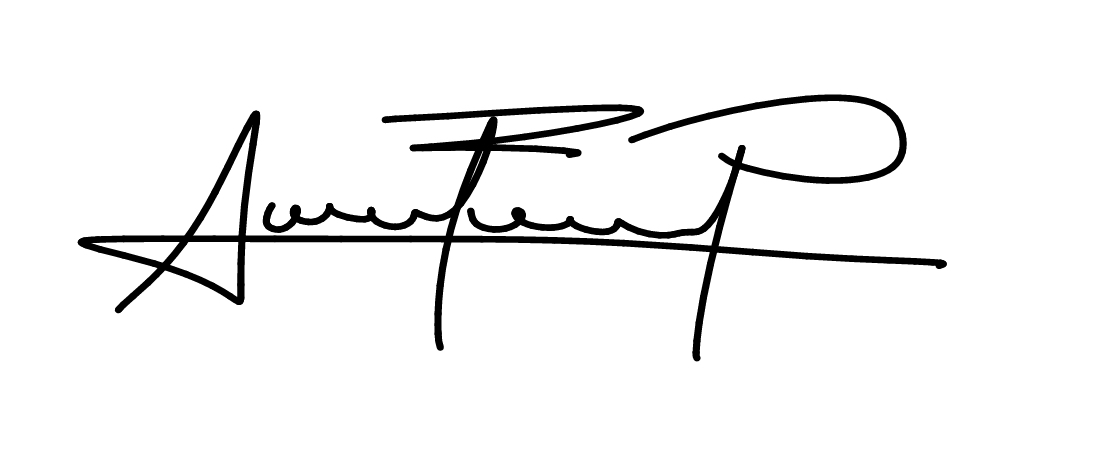
\includegraphics[width=4cm]{Imagenes/firma.jpg}

\vspace{-1.2cm}

\rule{7cm}{0.5pt}

\vspace{0.3cm}
\textbf{Andrés Felipe Pérez Sierra}\\
C.C. 1.108.206.142\\
Gerente General\\


\end{center}